\documentclass[../main.tex]{subfiles}

\chapter{Our Proposal: Spoof proof atomic clock controller}\label{op}
\begin{wrapfigure}{c}{0.45\textwidth}
  \centering
  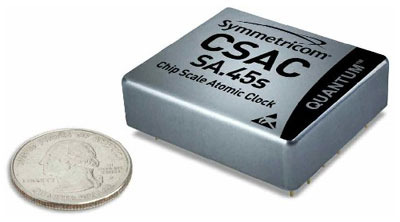
\includegraphics[width=0.40\textwidth]{csac.jpg}
  \caption[Symmetricom SA.45s CSAC]
   {Symmetricom SA.45s CSAC. Courtesy Symmetricom.}
\end{wrapfigure} 
We propose to construct and use what we call a \textit{Spoof proof atomic clock controller}. This is in essence just a piece of software running on a computer controlling a GPS disciplined atomic clock. The atomic clock serves two purposes:

\begin{itemize}
	\item Provide reference time to whatever application might need it.
	\item Provide data to the atomic clock controller in order for it to build a model of the atomic clock.
\end{itemize}

The computer running the atomic clock controller software will be connected to the atomic clock and perform the following trivial tasks:

\begin{itemize}
  \item Build and maintain the atomic clock model.
  \item Detecting abnormalities in atomic clock data and GPS data.
  \item Steer the atomic clock in case abnormalities.
\end{itemize}

Some of the point of the atomic clock atomic clock controller is to gain a situational awareness, being able to detect spoofing attacks, jamming and other abnormalities and or interferences. In our proposal, we use the term "filter" in context with this functionality. The term "filter" is used to describe an algorithm that can detect abnormal events by analyzing data collected during the events. A typical event could be a spoofing attack. Applying a filter to data collected during this event, should reveal the abnormality. Once an abnormal even has been detected, an action can be triggered.  The filters can be divided into two categories depending on their source of data comes. The GPS filters analyzes NMEA data from GPS receivers and atomic clock filters uses telemetry from the atomic clock.

\subsubsection{Atomic clock Model and filters}\label{csac_model_harald}
The atomic clock model is an algorithm used to predict what kind of behavior the atomic clock would exhibit given a set of data as input. It is used as a reference to determine the validity of the disciplining the atomic clock is subjected to. The atomic clock is disciplined by a 1 PPS signal generated by a GPS receiver. If that GPS receiver used for discipling is spoofed, the atomic clock model can be used to detect the spoofing. This is achieved by comparing the models predicted steer values being applied by the CSACs internal steer algorithms. The atomic clock model is the basis of all the atomic clock filters.

\subsubsection{GPS filter}\label{kvsrlf}
As discussed during the introduction (\ref{cspakp}), an easy way to detect spoofing, is to check the GPS receivers solved position against the known position of the receiver. The detection techniques efficiency also increases as more receivers are added to the detection setup. This is because it is hard to spoof a GPS receiver without also spoofing it's neighbor. By accidentally spoofing the neighbor, the two GPS receivers would solved the same position but different time (depending on the spoofing technique), thus giving away the attempt. 

\subsection{Note}
It is important to note that this approach doesn't really do anything with the fact that you are being attacked, it simply tries to eliminate the effects of it. In a scenario where you are under attack weeks at a time, you will have to address the fact that you are under attack at some point. It is also important to notes that this countermeasure mostly apply to applications using GPS as a source of time. Having a stable clock during a jamming attack will not help you determine your position once you move (given that you are fully jammed).